%\documentclass[handout,compress,xcolor=table]{beamer}
\usepackage{etex}
%\documentclass{article}
%\usepackage{beamerarticle}
\usepackage{tikz}
\usetikzlibrary{positioning,shapes,fit,arrows,shadows}
%\usepackage[turkish]{babel}
\usepackage[graph,arrow,curve,frame]{xy}
\usepackage[utf8]{inputenc}
\usepackage{listings}
\usepackage{multicol}
%\includeonlyframes{current}

\def\circtxt#1{$\mathalpha \bigcirc \mkern-13mu \mathtt #1$}
\def\smiley{\textcircled{\scriptsize $\mkern3mu\ddot{\ } \mkern-15mu \smallsmile$}}
\def\colorline#1{\cr \noalign{\color{#1} \hrule height 1pt \vskip-3em}}
\def\colorfline#1{\noalign{\color{#1} \hrule height 1pt}}
\def\OK{{\color{green!60!black}$\surd$}}
\def\NO{{\color{red!60!black}$\times$}}

\mode<article>
{
  \usepackage{fullpage}
  \usepackage{pgf}
  \usepackage{hyperref}
}

\mode<presentation>
{
  \usetheme{metuceng}

%  \setbeamercovered{transparent}
}


\title{Programming Language Concepts}
\subtitle{Syntax and Parsing}
\author{Onur Tolga Şehitoğlu}
\institute[ODTÜ]{Bilgisayar Mühendisliği}
\subject{Syntax and Parsing}
\date{}
	\titlegraphic{\insertmetutitle\insertlicense}


\begin{document}
\lstset{language=C,
        basicstyle=\scriptsize\ttfamily,
        keywordstyle=\color{blue!50!black}\bfseries,
        identifierstyle=\color{blue!60!green}\sffamily,
        stringstyle=\color{red!70!green}\ttfamily,
	commentstyle=\color{blue!30!white}\itshape,
        showstringspaces=true}
\setbeamercolor{hexample}{bg=green!5!white,fg=black}%
\setbeamercolor{cexample}{bg=blue!5!white,fg=black}%
\setbeamercolor{pexample}{bg=orange!5!white,fg=black}%
\setbeamercolor{oexample}{bg=violet!5!white,fg=black}%

 \frame[plain]{\maketitle}
 \begin{frame}
 \frametitle{Outline}
 \begin{multicols}{2}
 \tableofcontents
 \end{multicols}
 \end{frame}

\section{Describing Syntax}
\subsection{Introduction}
\begin{frame}
\frametitle{Introduction}
\begin{itemize}
\item \structure{Syntax}: the form and structure of a program.
\item \structure{Semantics}: meaning of a program
\item Language definitions are used by:
\begin{itemize}
\item Programmers
\item Implementors of the language processors
\item Language designers
\end{itemize}
\end{itemize}
\end{frame}

\begin{frame}
\frametitle{Definitions}
\begin{itemize}
\item A \structure{sentence}  is a string of characters over some alphabet
\item A \structure{language} is a set of sentences
\item A \structure{lexeme} is the lowest level syntactic unit of the language
	(i.e. \texttt{++, int, total})
\item A \structure{token} is a category of lexemes (i.e. \texttt{\em identifier\/})
\end{itemize}
\end{frame}


\begin{frame}
\frametitle{Definitions}
\begin{itemize}
\item \structure{syntax recognition}: read input strings of the language and verify the input belonging to the language
\item \structure{syntax generation}: generate sentences of the language (i.e. from a 
given data structure)
\item Compilers and interpreters recognize syntax and convert it into machine understandable form.
\end{itemize}
\end{frame}

\subsection{Backus-Naur Form and CFGs}
\begin{frame}
\frametitle{Backus-Naur Form and CFGs}
\begin{itemize}
\item CFG's introduced by Noam Chomsky (mid 1950s)
\item Programming languages are usually in \structure{context free language} class
\item BNF introduced by John Bakus and modified by Peter Naur for describing Algol language
\item BNF is equivalent to CFGs. It is a \structure{meta-language} that decribes other languages
\item Extended BNF improves readability of BNF
\end{itemize}
\end{frame}

\newcommand{\nt}[1]{$\langle${\bf #1}$\rangle$}
\begin{frame}
\frametitle{A Grammar Rule}
\texttt{\nt{while\_stmt} $\rightarrow$ while ( \nt{logic\_expr} ) \nt{stmt}}
\begin{itemize}
\item LHS is a non-terminal denoting an intermediate phrase
\item LHS can be defined (rewritten) as the RHS sequence which can contain
	terminals (lexems and tokens) of the language and other non-terminals
\item Non-terminals are denoted as strings enclosed in angle brackets.
\item \texttt{::=} may be used in BNF notation instead of the arrow
\item \texttt{$\mid$} is used to combine multiple rules with same LHS in a single rule\\
	\begin{minipage}[t]{.38\linewidth}
	\small
	\texttt{\nt{lgc\_cons} ::= true}\\
	\texttt{\nt{lgc\_cons} ::= false}\\
	\end{minipage} $\equiv$ \hfill
	\begin{minipage}[c]{.5\linewidth}
	\small
	\texttt{\nt{lgc\_cons} ::= true $\mid$ false }
	\end{minipage}
\end{itemize}
\end{frame}

\subsection{Context Free Grammar}
\begin{frame}
\frametitle{Context Free Grammar}
\begin{itemize}
\item A \structure{grammar} $G$ is defined as $G = (N, \Sigma , R, S)$:
\begin{itemize}
\item $N$, finite set of non terminals
\item $\Sigma$, finite set of terminals
\item $R$ is a set of grammar rules. A relation from $N$ to 
	$(N \cup \Sigma)^*$. 
\item $S \in N$ the  start symbol
\end{itemize}
\item Application of a rule maps one sentential form into the other
by replacing a non-terminal element in sentential form with
its right handside seuqence in the rule, $u \mapsto v$ .
\item Language of a grammar $L(G) = \left\{w \mid w \in \Sigma^{*},  S \stackrel{*}{\mapsto} w \right\}$
\end{itemize}
\end{frame}




\begin{frame}
\begin{itemize}
\item Recursive or list like structures can be represented using recursion\\
	\texttt{\nt{expr\_list} $\rightarrow$ \nt{expr} , \nt{expr\_list}} \\
	\texttt{\nt{btree} $\rightarrow$ \nt{head} ( \nt{btree} , \nt{btree} )}
\item A \structure{derivation} starts with a starting non-terminal and rules are applied repeteadly to end with a sentence containing only terminal symbols.
\item \structure{leftmost derivation}: always leftmost non-terminal is chosen for replacement
\item \structure{rightmost derivation}: always rightmost non-terminal is chosen for replacement
\item Same sentence can be derived using leftmost, rightmost, or other derivaionts.
\end{itemize}
\end{frame}

\begin{frame}
\frametitle{Sample Grammar}
{\small
~~~ \texttt{\nt{stmt} $\rightarrow$ \nt{id} = \nt{expr}}\\
~~~ \texttt{\nt{expr} $\rightarrow$ \nt{expr} \nt{op} \nt{expr} $\mid$ \nt{id}}\\
~~~ \texttt{\nt{op} $\rightarrow$ + $\mid$ *} \\
~~~ \texttt{\nt{id} $\rightarrow$ a $\mid$ b $\mid$ c}
}
\begin{itemize}
\item Leftmost derivation of \texttt{ a = a * b }:\\
{\texttt \small
\nt{stmt} $\mapsto$ \nt{id} = \nt{expr}
~ $\mapsto$ ~ a = \nt{expr}\\
~ $\mapsto$ ~ a = \nt{id} \nt{op} \nt{expr}
~ $\mapsto$ ~ a = a \nt{op} \nt{expr} \\
~ $\mapsto$ ~ a = a * \nt{expr}
~ $\mapsto$ ~ a = a * \nt{id}
~ $\mapsto$ ~ a = a * b}
\item Rightmost derivation of \texttt{ a = a * b }:\\
{\texttt \small
\nt{stmt} $\mapsto$ \nt{id} = \nt{expr} 
~ $\mapsto$ ~ \nt{id} = \nt{expr} \nt{op} \nt{expr} \\
~ $\mapsto$ ~ \nt{id} = \nt{expr} \nt{op} \nt{id}
~ $\mapsto$ ~ \nt{id} = \nt{expr} \nt{op} b \\
~ $\mapsto$ ~ \nt{id} = \nt{expr} * b
~ $\mapsto$ ~ \nt{id} = \nt{id} * b \\
~ $\mapsto$ ~ \nt{id} = a * b
~ $\mapsto$ ~ a = a * b
}
\end{itemize}
\end{frame}

\begin{frame}
\frametitle{Parse Tree}
\begin{itemize}
\item Steps of a derivation gives the structure of the sentence. This structure can be represented as a tree.
\item All non-terminals used in derivation are \structure{intermediate nodes}.
Each grammar rule replaces the non-terminal node with is children. Root node is the start symbol.
\item Terminal nodes are the \structure{leaf nodes}.
\item preorder traversal of leaf nodes gives the resulting sentence.
\item leftmost and rightmos derivations can be retrieved by traversal of the tree.
\end{itemize}
\end{frame}

\begin{frame}
\frametitle{Parse Tree Example}
\texttt{ a = a * b }\\
\centerline{
\xygraph{      []!{<14mm,0mm>:<0mm,8mm>::}
*+\txt{\nt{stmt}} 
	( :@{-}[dl] *+\txt{\nt{id}}
		( :@{-}[d] *+\txt{\tt a}
		) ,
	  :@{-}[d] *+\txt{\tt =} ,
   	    :@{-}[dr] *+\txt{\nt{expr}}
		( :@{-}[dl] *+\txt{\nt{expr}}
			( :@{-}[d] *+\txt{\nt{id}}
				( :@{-}[d] *+\txt{\tt a})),
		  :@{-}[d] *+\txt{\nt{op}}
			( :@{-}[d] *+\txt{\tt *}),
		  :@{-}[dr] *+\txt{\nt{expr}}
			( :@{-}[d] *+\txt{\nt{id}}
				( :@{-}[d] *+\txt{\tt b})
			)
		)
 	  )
}
}
\end{frame}

\begin{frame}
\frametitle{Parse Tree Generation}
\begin{itemize}
\item A parse tree gives the structure of the program so semantics
	of the program is related to this structure.
\item For example local scopes, evaluation order of expressions etc.
\item During compilation, parse trees might be required for 
code generation, semantic analysis and optimization phases.
\item After a parse tree generated, it can be traversed to 
	do various tasks of compilation.
\item The processing of parse tree takes too long, so creation
	of parse trees is usually avoided. 
\item Approaches like \structure{syntax directed translation} combines
	parsing with code generation, semantic analysis etc..
\end{itemize}
\end{frame}

\subsection{Ambigous Grammars}
\begin{frame}
\frametitle{Ambigous Grammars}
\begin{itemize}
\item Consider \texttt{a = a + b * c} in our grammar:\\
\begin{minipage}[t]{.4\linewidth}
\scriptsize
\xygraph{      []!{<7mm,0mm>:<0mm,7mm>::}
*+\txt{\nt{stmt}} 
	( :@{-}[dl] *+\txt{\nt{id}}
		( :@{-}[d] *+\txt{\tt a}
		) ,
	  :@{-}[d] *+\txt{\tt =} ,
   	  :@{-}[dr] *+\txt{\nt{expr}}
		( :@{-}[dl] *+\txt{\nt{expr}}
			( :@{-}[d] *+\txt{\nt{id}}
				( :@{-}[d] *+\txt{\tt a})),
		  :@{-}[d] *+\txt{\nt{op}}
			( :@{-}[d] *+\txt{\tt +}),
		  :@{-}[drr] *+\txt{\nt{expr}}
			( :@{-}[dl] *+\txt{\nt{expr}}
				( :@{-}[d] *+\txt{\nt{id}}
					( :@{-}[d] *+\txt{\tt b})),
			  :@{-}[d] *+\txt{\nt{op}}
				( :@{-}[d] *+\txt{\tt *}),
			  :@{-}[dr] *+\txt{\nt{expr}}
				( :@{-}[d] *+\txt{\nt{id}}
						( :@{-}[d] *+\txt{\tt c})
				)
			)
 	  )
} 
\end{minipage} ~ vs ~~
\begin{minipage}[t]{.45\linewidth}
\scriptsize
\xygraph{      []!{<8mm,0mm>:<0mm,8mm>::}
*+\txt{\nt{stmt}} 
	( :@{-}[dl] *+\txt{\nt{id}}
		( :@{-}[d] *+\txt{\tt a}
		) ,
	  :@{-}[d] *+\txt{\tt =} ,
   	  :@{-}[dr] *+\txt{\nt{expr}}
		(:@{-}[dl] *+\txt{\nt{expr}}
			( :@{-}[dl] *+\txt{\nt{expr}}
				( :@{-}[d] *+\txt{\nt{id}}
					( :@{-}[d] *+\txt{\tt a})),
			  :@{-}[d] *+\txt{\nt{op}}
				( :@{-}[d] *+\txt{\tt +}),
			  :@{-}[dr] *+\txt{\nt{expr}}
				( :@{-}[d] *+\txt{\nt{id}}
						( :@{-}[d] *+\txt{\tt b})
				)
			),
		  :@{-}[dr] *+\txt{\nt{op}}
			( :@{-}[d] *+\txt{\tt *}),
		  :@{-}[drr] *+\txt{\nt{expr}}
			( :@{-}[d] *+\txt{\nt{id}}
				( :@{-}[d] *+\txt{\tt c})) 
 	  )
}
\end{minipage}
\item
Both can be derived by the grammar!
\end{itemize}
\end{frame}

\begin{frame}
\begin{itemize}
\item A grammar is called \structure{ambigous} if same sentence can be
derived by following different set of rules, thus resulting in a different parse tree
\item If structure changes semantic meaning of the program, ambiguity is a serious problem.
\item Even if not, which one is the result?
\item i.e. Precedence of operators affects the value of the expression.
\item Programming languages enforces precedence rules to resolv
	ambiguity.
\item Solution:\\
	\begin{enumerate}
	\item design grammar not to be ambigous, or
	\item during parsing, choose rules to generate the correct parse tree
	\end{enumerate}
\end{itemize}
\end{frame}

\begin{frame}
\begin{itemize}
\frametitle{Precedence and Grammar}
\item Operators with different precedence levels should be treated differently
\item Higher precedence operations should be deep in the parse tree $\rightarrow$ their rules should be applied later.
\item Lower precedence operations should be closer to root $\rightarrow$ applied earlier in derivation.
\item  For each precedence level, define a non-terminal 
\item One rewritten on the other based on the precedence lower to higher
\end{itemize}
\end{frame}

\begin{frame}
\frametitle{Rewritten Grammar}
\begin{minipage}[t]{.5\linewidth}
{\scriptsize
\texttt{\nt{stmt} $\rightarrow$ \nt{id} = \nt{expr}}\\
\texttt{\nt{expr} $\rightarrow$ \nt{expr} + \nt{term} $\mid$ \nt{term}}\\
\texttt{\nt{term} $\rightarrow$ \nt{term} * \nt{factor} $\mid$ \nt{factor}}\\
\texttt{\nt{factor} $\rightarrow$ \nt{id} $\mid$ ( \nt{expr} ) } \\
\texttt{\nt{id} $\rightarrow$ a $\mid$ b $\mid$ c}
}
\end{minipage}
\begin{minipage}[t]{.4\linewidth}
\scriptsize
\xygraph{      []!{<7mm,0mm>:<0mm,6mm>::}
*+\txt{\nt{stmt}} 
	( :@{-}[dl] *+\txt{\nt{id}}
		( :@{-}[d] *+\txt{\tt a}
		) ,
	  :@{-}[d] *+\txt{\tt =} ,
   	  :@{-}[dr] *+\txt{\nt{expr}}
		( :@{-}[dl] *+\txt{\nt{expr}}
			( :@{-}[d] *+\txt{\nt{term}}
			( :@{-}[d] *+\txt{\nt{factor}}
			( :@{-}[d] *+\txt{\nt{id}}
				( :@{-}[d] *+\txt{\tt a})))),
		  :@{-}[d] *+\txt{\tt +},
		  :@{-}[drr] *+\txt{\nt{term}}
			( :@{-}[dl] *+\txt{\nt{term}}
				( :@{-}[d] *+\txt{\nt{factor}}
				   	(:@{-}[d] *+\txt{\nt{id}}
					( :@{-}[d] *+\txt{\tt b}))
				),
			  :@{-}[d] *+\txt{\texttt{*}},
			  :@{-}[dr] *+\txt{\nt{factor}}
				( :@{-}[d] *+\txt{\nt{id}}
						( :@{-}[d] *+\txt{\tt c})
				)
			)
 	  )
} 
\end{minipage}
\begin{itemize}
\item \nt{term} and \nt{expr} has different precedence.
\item Once inside of \nt{term}, there is no way to derive \texttt{+}
\item Only one parse possible
\end{itemize}
\end{frame}

\subsection{Associativity}
\begin{frame}
\frametitle{Associativity}
\begin{itemize}
\item Associativity of operators is another issue\\ 
{\tt a - b - c $\equiv$ ( a - b ) - c  ~ \textrm{or} ~  a - ( b - c)}
\item  Recursion of grammar defines how tree is constructed for operators
	in the  same level.
\item If left recursive, later operators in the sentence will be closer to
	root, if right recursive earlier operators will be closer to root
\item \structure{left recursion} implies left associativity, \structure{right
	recursion} implies right associativity.
\item Consider \texttt{\small a + b + c} in these grammars:\\
\begin{tabular}{lll}
\begin{minipage}{.4\linewidth}
\scriptsize
\texttt{\nt{expr} $\rightarrow$ \nt{expr} + \nt{id} $\mid$ \nt{id}}\\
\texttt{\nt{id} $\rightarrow$ a $\mid$ b $\mid$ c}
\end{minipage}
& vs &
\begin{minipage}{.4\linewidth}
\scriptsize
\texttt{\nt{expr} $\rightarrow$ \nt{id} + \nt{expr} $\mid$ \nt{id}}\\
\texttt{\nt{id} $\rightarrow$ a $\mid$ b $\mid$ c}
\end{minipage}
\end{tabular}
\end{itemize}
\end{frame}

\subsection{An Assignment Grammar}
\begin{frame}
\frametitle{Sample Grammar}
{\scriptsize
~~~~~ \texttt{\nt{asgn} $\rightarrow$ \nt{id} = \nt{asgn} $\mid$ \nt{id} = \nt{expr}}\\
~~~~~ \texttt{\nt{expr} $\rightarrow$ \nt{expr} + \nt{term} $\mid$ \nt{term}}\\
~~~~~ \texttt{\nt{term} $\rightarrow$ \nt{term} * \nt{factor} $\mid$ \nt{factor}}\\
~~~~~ \texttt{\nt{factor} $\rightarrow$ \nt{pow} \lstinline'^' \nt{factor} $\mid$ \nt{pow}}\\
~~~~~ \texttt{\nt{pow} $\rightarrow$ \nt{id} $\mid$ ( \nt{expr} ) } \\
~~~~~ \texttt{\nt{id} $\rightarrow$ a $\mid$ b $\mid$ c} \\[1cm]

\begin{itemize}
\item \nt{asgn} is right recursive like right associative C assignments.
\item \nt{expr} and \nt{term} are left recursive, {\tt *} and {\tt +} left 
	associative
\item \nt{factor} is right recursive for power operation \lstinline{^}
	to be right associative.
\item precedence order is {\tt ($...$) $\prec$ \lstinline!^! $\prec$ * 
	$\prec$  + $\prec$ =}
\end{itemize}
}
\end{frame}

\begin{frame}
\  
{\small \tt a = a + b * c * a \lstinline!^! b \lstinline!^! c}\ \\[5mm]
\scriptsize
\xygraph{[]!{<7mm,0mm>:<0mm,7mm>::}
*+\txt{\nt{asgn}}
(
   :@{-}[dl] *+\txt{\nt{id}}
   (
      :@{-}[d] *+\txt{\tt a}
   ) ,
   :@{-}[d] *+\txt{\tt =} ,
   :@{-}[drrrr] *+\txt{\nt{expr}}
   (
      :@{-}[dlll] *+\txt{\nt{expr}}
      (
         :@{-}[d] *+\txt{\nt{term}}
         (
            :@{-}[d] *+\txt{\nt{factor}}
            (
               :@{-}[d] *+\txt{\nt{pow}}
               (
                  :@{-}[d] *+\txt{\nt{id}}
                  (
                     :@{-}[d] *+\txt{\tt a}
                  )
               )
            )
         )
      ) ,
      :@{-}[d] *+\txt{\tt +} ,
      :@{-}[drrr] *+\txt{\nt{term}}
      (
         :@{-}[dll] *+\txt{\nt{term}}
         (
            :@{-}[dl] *+\txt{\nt{term}}
            (
               :@{-}[d] *+\txt{\nt{factor}}
               (
                  :@{-}[d] *+\txt{\nt{pow}}
                  (
                     :@{-}[d] *+\txt{\nt{id}}
                     (
                        :@{-}[d] *+\txt{\tt b}
                     )
                  )
               )
            ) ,
            :@{-}[d] *+\txt{\tt *} ,
            :@{-}[dr] *+\txt{\nt{factor}}
            (
               :@{-}[d] *+\txt{\nt{pow}}
               (
                  :@{-}[d] *+\txt{\nt{id}}
                  (
                     :@{-}[d] *+\txt{\tt c}
                  )
               )
            )
         ) ,
         :@{-}[d] *+\txt{\tt *} ,
         :@{-}[drr] *+\txt{\nt{factor}}
         (
            :@{-}[dl] *+\txt{\nt{pow}}
            (
               :@{-}[d] *+\txt{\nt{id}}
               (
                  :@{-}[d] *+\txt{\tt a}
               )
            ) ,
            :@{-}[d] *+\txt{\tt \lstinline!^!} ,
            :@{-}[dr] *+\txt{\nt{factor}}
            (
               :@{-}[dl] *+\txt{\nt{pow}}
               (
                  :@{-}[d] *+\txt{\nt{id}}
                  (
                     :@{-}[d] *+\txt{\tt b}
                  )
               ) ,
               :@{-}[d] *+\txt{\tt \lstinline!^!} ,
               :@{-}[dr] *+\txt{\nt{factor}}
               (
                  :@{-}[d] *+\txt{\nt{pow}}
                  (
                     :@{-}[d] *+\txt{\nt{id}}
                     (
                        :@{-}[d] *+\txt{\tt c}
                     )
                  )
               )
            )
         )
      )
   )
)
}
\end{frame}

\subsection{if-then-else ambiguity}
\begin{frame}
\frametitle{if-then-else ambiguity}
\begin{itemize}
\item Following grammar is ambigous:\\
{\scriptsize
~~~~~ \texttt{\nt{stmt} $\rightarrow$ \nt{if-stmt}}\\
~~~~~ \texttt{\nt{if-stmt} $\rightarrow$ 
		 	      if \nt{logic-expr} then \nt{stmt}  $\mid$}\\
~~~~~~~~~~~~~~~~~~~~~~ \texttt{if \nt{logic-expr} then \nt{stmt} else 
					\nt{stmt}}\\
}
\item Consider \texttt{if a then if b then x=1 else x=0}:\\
\only<2-3>{
\begin{minipage}[t]{.45\linewidth}
\scriptsize
\xygraph{      []!{<8mm,0mm>:<0mm,8mm>::}
*+\txt{\nt{if-stmt}} 
	( :@{-}[dl] *+\txt{\tt if},
	  :@{-}[ddl] *+\txt{\nt{logic-expr}}
	   ( :@{.}[dl] *+\txt{\tt a}),
	  :@{-}[d] *+\txt{\tt then} ,
   	  :@{-}[ddr] *+\txt{\nt{stmt}}
   	  (:@{-}[d] *+\txt{\nt{if-stmt}}
		(:@{-}[dll] *+\txt{\tt if},
	  	:@{-}[ddl] *+\txt{\nt{logic-expr}} 
		( :@{.}[d] *+\txt{\tt b}),
	  	:@{-}[d] *+\txt{\tt then} ,
   	  	:@{-}[dr] *+\txt{\nt{stmt}}
		( :@{.}[d] *+\txt{\tt x=1})
		)
	  ),
   	  :@{-}[dr] *+\txt{\tt else},
   	  :@{-}[drr] *+\txt{\nt{stmt}}
		( :@{.}[d] *+\txt{\tt x=0})
} 
\end{minipage}  ~ vs ~}
\only<3-3>{
\begin{minipage}[t]{.45\linewidth}
\scriptsize
\xygraph{      []!{<8mm,0mm>:<0mm,8mm>::}
*+\txt{\nt{if-stmt}} 
	( :@{-}[dl] *+\txt{\tt if},
	  :@{-}[ddl] *+\txt{\nt{logic-expr}}
	   ( :@{.}[d] *+\txt{\tt a}),
	  :@{-}[d] *+\txt{\tt then} ,
	  :@{-}[dr] *+\txt{\nt{stmt}} (
   	  :@{-}[d] *+\txt{\nt{if-stmt}}
		(:@{-}[dl] *+\txt{\tt if},
	  	   :@{-}[ddl] *+\txt{\nt{logic-expr}} 
		      ( :@{.}[d] *+\txt{\tt b}),
	  	   :@{-}[d] *+\txt{\tt then} ,
   	  	   :@{-}[ddr] *+\txt{\nt{stmt}}
		      ( :@{.}[d] *+\txt{\tt x=1}),
		   :@{-}[dr] *+\txt{\tt else},
		   :@{-}[drr] *+\txt{\nt{stmt}}
			( :@{.}[d] *+\txt{\tt x=0})
		)
	   )
	)
}
\end{minipage}}
\end{itemize}
\end{frame}

\begin{frame}
\frametitle{Solution}
\begin{itemize}
\item Distinguish categories of statements. if's matched with else and unmatched:\\
{\scriptsize
~~~~~ \texttt{\nt{stmt} $\rightarrow$ \nt{matched} $\mid$ \nt{unmatched}}\\
~~~~~ \texttt{\nt{matched} $\rightarrow$ 
		 	      if \nt{logic-expr} then \nt{matched} else
				\nt{matched} $\mid$}\\
~~~~~~~~~~~~~~~~~~~~~~ \texttt{\nt{other-stmt}} \\
~~~~~ \texttt{\nt{unmatched} $\rightarrow$ 
		 	      if \nt{logic-expr} then \nt{stmt} $\mid$}\\
~~~~~~~~~~~~~~~~~~~~~~ \texttt{if \nt{logic-expr} then \nt{matched} else
                                \nt{unmatched}} \\
}
\item \texttt{if a then if b then x=1 else x=0}:\\
\only<2-2>{\tiny
\xygraph{      []!{<10mm,0mm>:<0mm,6mm>::}
*+\txt{\nt{unmatched}} 
	( :@{-}[dl] *+\txt{\tt if},
	  :@{-}[ddl] *+\txt{\nt{logic-expr}}
	   ( :@{.}[d] *+\txt{\tt a}),
	  :@{-}[d] *+\txt{\tt then} ,
	  :@{-}[dr] *+\txt{\nt{stmt}} (
   	  :@{-}[d] *+\txt{\nt{matched}}
		(:@{-}[dl] *+\txt{\tt if},
	  	   :@{-}[ddl] *+\txt{\nt{logic-expr}} 
		      ( :@{.}[d] *+\txt{\tt b}),
	  	   :@{-}[d] *+\txt{\tt then} ,
   	  	   :@{-}[ddr] *+\txt{\nt{matched}}
		      ( :@{.}[d] *+\txt{\tt x=1}),
		   :@{-}[dr] *+\txt{\tt else},
		   :@{-}[drr] *+\txt{\nt{matched}}
			( :@{.}[d] *+\txt{\tt x=0})
		)
	   )
	)
}
}
\end{itemize}
\vspace{10em}
\end{frame}

\defverbatim[colored]\codesource{
\begin{minipage}{.35\textwidth}
\begin{lstlisting}[language={C},basicstyle=\tiny\ttfamily]
while (counter < 12341) { 
	f() ; 
	counter += 12;
}
\end{lstlisting}\end{minipage}}
\defverbatim[colored]\codelexsrc{
\begin{minipage}{.35\textwidth}
\begin{lstlisting}[language={C},basicstyle=\tiny\ttfamily]
WHL LP ID LT ILIT RP LB
	ID LP RP SC
	ID PLEQ ILIT SC
RB
\end{lstlisting}\end{minipage}}
\defverbatim[colored]\codemachine{\begin{minipage}{.35\textwidth}
\begin{lstlisting}[language={C},basicstyle=\tiny\ttfamily]
001f 0001 0006 0000 
0034 0021 0000 0000 
0004 0000 001b 0009 
0000 0000 02f4 0008 
0008 0001 0004 0008 
0025 0001 0003 0000 
0058 0000 0000 0000 
0004 0000 002b 0008 
\end{lstlisting}\end{minipage}}
\defverbatim[colored]\codeasm{\begin{minipage}{.35\textwidth}
\begin{lstlisting}[language={[x86masm]Assembler},basicstyle=\tiny\ttfamily]
.L3:
	movl	$0, %eax
	call	f
	addl	$12, -4(%rbp)
.L2:
	cmpl	$12340, -4(%rbp)
	jle	.L3
	leave
	ret
\end{lstlisting}\end{minipage}}

\newcommand{\lblst}[1]{\tiny\rm \color{red!70!green}{#1}}
\newcommand{\CNODE}[1]{%
	\begin{minipage}{15mm} \centering%
	\tiny #1%
	\end{minipage}%
	}
\section{Parsing}
\subsection{Compilation}
\begin{frame}
\frametitle{Compilation}
\begin{columns}
\begin{column}{.6\textwidth} \scriptsize
\hspace*{1em}
\begin{tikzpicture} [ stbox/.style={draw,top color=blue!20!white,bottom color=blue!5!white,rectangle,
						drop shadow,rounded corners=2pt},
				    label2/.style={fill=white},
				    label3/.style={fill=white},
				    label4/.style={fill=white},
				    label5/.style={fill=white},
				    label1/.style={fill=white},
					conn/.style={thick}]
\only<1-1>{\tikzset{label1/.style={green!90!white,fill=white}
				  }}
\only<2-2>{\tikzset{label2/.style={green!90!white,fill=white}
				  }}
\only<3-3>{\tikzset{label3/.style={green!90!white,fill=white}
				  }}
\matrix [column sep=5mm,ampersand replacement=\&] {
	\& \node (CSTART) {}; \\[8mm]
	\& \node [stbox] (CLA) {\CNODE{Lexical Analysis}};	\\[8mm]
	\& \node [stbox] (CSA) {\CNODE{Syntax analysis}}; \\ [8mm]
\node [top color=green!90!white, rectangle,draw, bottom color=green!40!white] (CST) { \begin{minipage}{8mm} \centering
\tiny Symbol Table
\end{minipage}}; \&
	\node [stbox] (CIC) {\CNODE{Intermediate code generation and Semantic Analysis}};
		\& \node [stbox] (COP) {\CNODE{Optimization}}; \\ [8mm]
	\& \node [stbox] (CCG) {\CNODE{Code generation}}; \\[8mm]
\& \node (CEND) {};\\
};
\draw [conn,->] (CSTART) -- node [label1] {\tiny source code} (CLA); 	
\draw [conn,->] (CLA) -- node [label2] {\tiny sequence of lexemes} (CSA);
\draw [conn,->] (CSA) -- node [label3] {\tiny parse tree} (CIC);
\draw [conn,->] (CST) -- (CIC);		
\draw [conn,->] (CLA) -| (CST);
\draw [conn,->] (CSA) -| (CST);
\draw [conn,->] (CIC) -- node [label4] {\tiny intermediate code} (CCG);
\draw [conn,->] (CIC) -- (COP);
\draw [conn,->] (COP) -- (CIC);
\draw [conn,->] (CCG) -- node [label5] {\tiny machine code} (CEND);	
\end{tikzpicture}
\end{column}
\begin{column}{.6\textwidth} \scriptsize
\only<1-1>{\codesource\ \\}%
\only<2-2>{\codelexsrc\ \\}%
\only<3-3>{\tiny\xygraph{[]!{<6mm,0mm>:<0mm,6mm>::} %
*+\txt{\nt{whlstmt}}  %
	(  :@{-}[dlll] *+\txt{\tt  WHL} , %
	   :@{-}[dl] *+\txt{\nt{lgcexp}} %
		( :@{-}[dl] *+\txt{\nt{expr}}
			( :@{-}[d] *+\txt{\nt{id}}
				( :@{-}[d] *+\txt{\tt ID} )),
		  :@{-}[d] *+\txt{\nt{cmp}}
		  	( :@{-}[d] *+\txt{\tt LT} ),
		  :@{-}[dr] *+\txt{\nt{expr}}
			( :@{-}[d] *+\txt{\nt{lit}}
				( :@{-}[d] *+\txt{\tt ILIT} ))
		) , %
 	  :@{-}[drr] *+\txt{\nt{stmt}} ( :@{-}[dl] *+\txt{\tt LB},
		  :@{-}[d] *+\txt{\nt{stmtlst}}
			( :@{-}[dl] *+\txt{\nt{stmt}}
				( :@{-}[d] *+\txt{\nt{call}}
				( :@{-}[dl] *+\txt{\nt{id}}
					( :@{-}[d] *+\txt{\tt ID} )	,
			  	  :@{-}[d] *+\txt{\tt LP},
			  	  :@{-}[dr] *+\txt{\nt{prms}}
					( :@{-}[d] *+{ \epsilon}),
			  	  :@{-}[drr] *+\txt{\tt RP}
				)
				)	,
			  :@{-}[d] *+\txt{\tt SC},
			  :@{-}[dr] *+\txt{\nt{stmtlst}}
				(:@{-}[dr] *+\txt{\tt ...})
			),
		  :@{-}[dr] *+\txt{\tt RB}
		)
	) %
}}
\end{column}
\end{columns}
\end{frame}

\begin{frame}
\frametitle{Compilation}
\begin{columns}
\begin{column}{.6\textwidth} \scriptsize
\hspace*{1em}
\begin{tikzpicture} [ stbox/.style={draw,top color=blue!20!white,bottom color=blue!5!white,rectangle,
						drop shadow,rounded corners=2pt},
				    label2/.style={fill=white},
				    label3/.style={fill=white},
				    label4/.style={fill=white},
				    label5/.style={fill=white},
				    label1/.style={fill=white},
					conn/.style={thick}]
\only<1-1>{\tikzset{label4/.style={green!90!white,fill=white}
				  }}
\only<2-2>{\tikzset{label5/.style={green!90!white,fill=white}
				  }}
\matrix [column sep=5mm,ampersand replacement=\&] {
	\& \node (CSTART) {}; \\[8mm]
	\& \node [stbox] (CLA) {\CNODE{Lexical Analysis}};	\\[8mm]
	\& \node [stbox] (CSA) {\CNODE{Syntax analysis}}; \\ [8mm]
\node [top color=green!90!white, rectangle,draw, bottom color=green!40!white] (CST) { \begin{minipage}{8mm} \centering
\tiny Symbol Table
\end{minipage}}; \&
	\node [stbox] (CIC) {\CNODE{Intermediate code generation and Semantic Analysis}};
		\& \node [stbox] (COP) {\CNODE{Optimization}}; \\ [8mm]
	\& \node [stbox] (CCG) {\CNODE{Code generation}}; \\[8mm]
\& \node (CEND) {};\\
};
\draw [conn,->] (CSTART) -- node [label1] {\tiny source code} (CLA); 	
\draw [conn,->] (CLA) -- node [label2] {\tiny sequence of lexemes} (CSA);
\draw [conn,->] (CSA) -- node [label3] {\tiny parse tree} (CIC);
\draw [conn,->] (CST) -- (CIC);		
\draw [conn,->] (CLA) -| (CST);
\draw [conn,->] (CSA) -| (CST);
\draw [conn,->] (CIC) -- node [label4] {\tiny intermediate code} (CCG);
\draw [conn,->] (CIC) -- (COP);
\draw [conn,->] (COP) -- (CIC);
\draw [conn,->] (CCG) -- node [label5] {\tiny machine code} (CEND);	
\end{tikzpicture}
\end{column}
\begin{column}{.6\textwidth} \scriptsize
\only<1-1>{\codeasm}
\only<2-2>{\codemachine}
\end{column}
\end{columns}
\end{frame}


\subsection{Lexical Analysis}
\begin{frame}
\frametitle{Lexical Analysis}
\begin{itemize}
\item \structure{input}: sequence of characters, source code.
\item \structure{output}: sequence of lexemes
\item Worst case complexity of parsing is ${\cal O}(n^3)$.
	Depending on algorithm type, recursion type and number of
	grammar rules, this might change. $n$ is the length of the string.
\item Regular language processing complexity is ${\cal O}(n)$. Grammars can be 
	defined in terms of lexemes.
\item \# of chars vs \# of lexemes? 
\item Lexical analysis convert character sequences into lexemes. Identifiers
	registered on symbol table
\end{itemize}
\end{frame}

\subsection{Parsing}
\begin{frame}
\frametitle{Parsing}
\begin{itemize}
\item \structure{input}: sequence of lexemes (output of lexical analysis) or characters.
\item \structure{output}: parse tree, intermediate code, translated code, or sometimes only if document is valid or not.
\item Two main classes of parser:
	\begin{itemize}
	\item Top down parsing
	\item Tottom up parsing
	\end{itemize}
\end{itemize}
\end{frame}

\subsection{Top-down Parsing}
\begin{frame}
\frametitle{Top-down Parsing}
\begin{itemize}
\item Start from the starting non-terminal, apply grammar rules to 
	reach the input sentence 
	{\small
	\[ \begin{array}{l}
	\langle assign \rangle ~~ \mapsto
	~~ a = \langle expr\rangle  ~~ \mapsto
	~~ a = \langle expr\rangle + \langle term\rangle  ~~ \mapsto \\
	~~ a = \langle term\rangle + \langle term\rangle  ~~ \mapsto
	~~ a = \langle fact \rangle + \langle term\rangle  ~~ \mapsto \\
	~~ a = a + \langle term\rangle  ~~ \mapsto 
	~~ a = a + \langle term\rangle * \langle fact\rangle  ~~ \mapsto \\
	~~ a = a + \langle fact\rangle * \langle fact\rangle  ~~ \mapsto 
	~~ a = a + b * \langle fact\rangle  ~~ \mapsto  \\
	~~ a = a + b * a  
\end{array}
	\]}
\item Simplest form gives leftmost derivation of a grammar processing input
	from left to right.
\item Left recursion in grammar is a problem. Elimination of left recursion
	needed.
\item \structure{Deterministic parsing:} Look at input symbols to choose next
	rule to apply.
\item \structure{recursive descent parsers}, \structure{LL} family parsers 
	are top-down parsers
\end{itemize}
\end{frame}

\defverbatim[colored]\coderdparser{
\begin{lstlisting}[language={C}]
typedef enum {ident, number, lparen, rparen, times, 
	slash, plus, minus} Symbol;
int accept(Symbol s) { if (sym == s) { next(); return 1; } 
	return 0;
}
void factor(void) {
    if (accept(ident)) ;
    else if (accept(number)) ;
    else if (accept(lparen)) { expression(); expect(rparen);}
    else { error("factor: syntax error at ",currsym); next(); }
}
void term(void) {
    factor();
    while (accept(times) || accept(slash))
        factor();
}
void expression(void) {
    term();
    while (accept(plus) || accept(minus))
        term();
}
\end{lstlisting}}
\begin{frame}
\subsection{Recursive Descent Parser}
\frametitle{Recursive Descent Parser}
\begin{beamercolorbox}{cexample}
\coderdparser
\end{beamercolorbox}
\end{frame}

\begin{frame}
\begin{itemize}
\item Each non-terminal realized as a parsing function
\item Parsing functions calls the right handside functions in sequence
\item Rule choices are based on the current input symbol. \texttt{accept}
	checks a terminal and consumes if matches.
\item Cannot handle direct or indirect left recursion. A function has to call 
	itself before anything else.
\item Hand coded, not flexible.
\end{itemize}
\end{frame}

\begin{frame}
\subsection{LL Parsers}
\frametitle{LL Parsers}
\begin{itemize}
\item First L is `left to right input processing', second is 
	`leftmost derivation'
\item Checks next $N$ input symbols to decide on which rule to apply: LL($N$) parsing.
\item For example LL(1) checks the next input symbol only.
\item LL($N$) parsing table: A table for $V \times \Sigma^{N} \mapsto R$
\item for expanding a nonterminal $NT \in V$, looking at this table and the next $N$ input symbols, LL($N$) parser chooses the grammar rule $r \in R$ to apply in the next step.
\end{itemize}
\end{frame}

\begin{frame}
\begin{itemize}
\item Grammar and lookup table for a LL(1) parser:
\begin{minipage}[c]{.4\linewidth}
\small
\[
 \begin{array}{ll}
\mathrm{1} &	S \rightarrow E \\
\mathrm{2} &	S \rightarrow \mathtt{-} E \\
\mathrm{3} &	E \rightarrow  N \mathtt{+} E \\
\mathrm{4} &	E \rightarrow \mathtt{(} E \mathtt{)} \\
\mathrm{5} &	N \rightarrow \mathtt{a} \\
\mathrm{6} &	N \rightarrow \mathtt{b} \\
 \end{array}
 \]
\end{minipage}
\begin{tabular}{|>{\columncolor{blue!10} }l|c|c|c|c|} \rowcolor{blue!20} \hline
	& a 	& b 	& - 	& {\tt (} \\ \hline \hline
S	& 1	& 1	& 2	& 1  \\	\hline
E	& 3 	& 3	&	& 4  \\\hline
N	& 5	& 6	&	&    \\\hline
\end{tabular}
\item What if we add {\small $E \rightarrow N$} to grammar? 
\item You need an LL(2) grammar. What if $N$ is recursive?\\
	\only<2-2>{see LL(*) parser}
\end{itemize}
\end{frame}

\subsection{Bottom-up Parsing}
\begin{frame}
\frametitle{Bottom-up Parsing}
\begin{itemize}
\item Start from input sentence and merge parts of sentential form matching RHS of a rule into LHS at each step. Try to reach the starting non-terminal.
	reach the input sentence \\ {\small
	\[ \begin{array}{l}
	~~ a = a + b * a  ~~ \mapsto
	~~ a = \langle fact \rangle + b * a  ~~ \mapsto 
	~~ a = \langle term\rangle + b * a  ~~ \mapsto \\
	~~ a = \langle expr\rangle + b * a  ~~ \mapsto
	~~ a = \langle expr\rangle + \langle fact\rangle * a  ~~ \mapsto \\
	~~ a = \langle expr\rangle + \langle term\rangle * a  ~~ \mapsto
	~~ a = \langle expr\rangle + \langle term\rangle * \langle fact\rangle  ~~ \mapsto \\
	~~ a = \langle expr\rangle + \langle term\rangle ~~ \mapsto
	~~ a = \langle expr\rangle ~~ \mapsto
	\langle assign \rangle 
\end{array}
	\]}
\item Simplest form gives rightmost derivation of a grammar (in reverse) processing input
	from left to right.
\item Shift-reduce parsers are bottom-up:
	\begin{itemize}
	\item \structure{shift:} take a symbol from input and push to stack.
	\item \structure{reduce:} match and pop a RHS from stack and reduce into	
	LHS.
	\end{itemize}
\end{itemize}
\end{frame}


\defverbatim[colored]\codeshiftreduce{
\begin{lstlisting}[language=Prolog,escapechar=\#]
% Grammar is E-> E-T|E+T|T  T -> a|b
rule(e,[e,-,t]).
rule(e,[e,+,t]).
rule(e,[t]).
rule(t,[a]).
rule(t,[b]).

parse([],[S]) :- S = e .  % starting symbol alone in the stack
% reduce: find RHS of a rule on stack, reduce it to LHS
parse(Input,Stack) :- match(LHS,Stack,Remainder), 
		      parse(Input,[LHS|Remainder]).

% shift: nonterminals are removed from input added on stack
parse([H|Input],Stack) :- member(X,[a,b,-,+]),
	 		  parse(Input,[H|Stack]).

% check if RSH of a rule is a prefix of Stack (reversed).
match(LHS,List,L) :- rule(LHS,RHS),  reverse(RHS,NRHS),
	 	     prefix(NRHS,List,L).
\end{lstlisting}}
\begin{frame}
\frametitle{Shift-Reduce Parser in Prolog}
\begin{beamercolorbox}{oexample}
\codeshiftreduce
\end{beamercolorbox}
\end{frame}

\begin{frame}
\begin{itemize}
\item Shift reduce parser tries all non-deterministic shift combinations to get all
	parses.
\item For deterministic parsing states based on input lookahead or
	precedence required
\item Deterministic bottom up parsers: LALR, SLR(1).
\end{itemize}
\end{frame}
\end{document}
